\documentclass{beamer}
\usepackage[utf8]{inputenc}
\usepackage{graphicx, epsfig}
\usepackage{amsmath,mathrsfs,amsfonts,amssymb}
\usepackage{floatflt}
\usepackage{epic,ecltree}
\usepackage{mathtext}
\usepackage{fancybox}
\usepackage{fancyhdr}
\usepackage{multirow}
\usepackage{enumerate}
\usepackage{epstopdf}
\usepackage{multicol}
\usepackage{algorithm}
\usepackage[noend]{algorithmic}
\usepackage{tikz}
\usepackage{blindtext}
\usetheme{default}%{Singapore}%{Warsaw}%{Warsaw}%{Darmstadt}
\usecolortheme{default}

\setbeamerfont{title}{size=\Huge}
\setbeamertemplate{footline}[page number]{}

\setbeamertemplate{section in toc}[sections numbered]


\makeatletter
\newcommand\HUGE{\@setfontsize\Huge{35}{40}}
\makeatother    

\setbeamerfont{title}{size=\HUGE}
\beamertemplatenavigationsymbolsempty

% latin bold lower
\newcommand{\ba}{\mathbf{a}} 
\newcommand{\bc}{\mathbf{c}} 
\newcommand{\be}{\mathbf{e}} 
\newcommand{\bh}{\mathbf{h}} 
\newcommand{\bp}{\mathbf{p}} 
\newcommand{\bt}{\mathbf{t}} 
\newcommand{\bs}{\mathbf{s}} 
\newcommand{\bu}{\mathbf{u}} 
\newcommand{\bv}{\mathbf{v}} 
\newcommand{\bw}{\mathbf{w}} 
\newcommand{\bx}{\mathbf{x}} 
\newcommand{\by}{\mathbf{y}} 
\newcommand{\bz}{\mathbf{z}} 

% latin bold upper
\newcommand{\bA}{\mathbf{A}} 
\newcommand{\bB}{\mathbf{B}} 
\newcommand{\bC}{\mathbf{C}} 
\newcommand{\bI}{\mathbf{I}} 
\newcommand{\bL}{\mathbf{L}} 
\newcommand{\bM}{\mathbf{M}} 
\newcommand{\bQ}{\mathbf{Q}} 
\newcommand{\bT}{\mathbf{T}} 
\newcommand{\bU}{\mathbf{U}} 
\newcommand{\bV}{\mathbf{V}} 
\newcommand{\bW}{\mathbf{W}} 
\newcommand{\bX}{\mathbf{X}} 
\newcommand{\bY}{\mathbf{Y}} 
\newcommand{\bZ}{\mathbf{Z}} 

% latin cal upper
\newcommand{\cG}{\mathcal{G}} 
\newcommand{\cL}{\mathcal{L}} 
\newcommand{\cN}{\mathcal{N}} 
\newcommand{\cS}{\mathcal{S}} 
\newcommand{\cT}{\mathcal{T}} 
\newcommand{\cW}{\mathcal{W}} 
\newcommand{\cX}{\mathcal{X}} 
\newcommand{\cZ}{\mathcal{Z}} 

% latin bb upper
\newcommand{\bbE}{\mathbb{E}} 
\newcommand{\bbI}{\mathbb{I}} 
\newcommand{\bbP}{\mathbb{P}} 
\newcommand{\bbR}{\mathbb{R}} 

% greek bold lower
\newcommand{\bepsilon}{\boldsymbol{\epsilon}} 
\newcommand{\btheta}{\boldsymbol{\theta}} 
\newcommand{\blambda}{\boldsymbol{\lambda}} 
\newcommand{\bpi}{\boldsymbol{\pi}} 
\newcommand{\bmu}{\boldsymbol{\mu}} 
\newcommand{\bsigma}{\boldsymbol{\sigma}} 
\newcommand{\bphi}{\boldsymbol{\phi}} 

% greek bold upper
\newcommand{\bSigma}{\boldsymbol{\Sigma}} 

\DeclareMathOperator*{\argmin}{arg\,min}
\DeclareMathOperator*{\argmax}{arg\,max}

\newcommand{\createdgmtitle}[1]{\title[\hbox to 56mm{Deep Generative Models  \hfill\insertframenumber\,/\,\inserttotalframenumber}]
	{Deep Generative Models \\ {\Huge Lecture #1}}
	\author{Roman Isachenko}
	\institute{
\includegraphics[width=0.5cm]{../utils/ozonmasterslogo} \large{Ozon Masters}}
	\date{Spring, 2022}
}

\newcommand\myfootnote[1]{%
  \tikz[remember picture,overlay]
  \draw (current page.south west) +(1in + \oddsidemargin,0.5em)
  node[anchor=south west,inner sep=0pt]{\parbox{\textwidth}{%
      \rlap{\rule{10em}{0.4pt}}\raggedright\scriptsize \textit{#1}}};}

\newcommand\myfootnotewithlink[2]{%
  \tikz[remember picture,overlay]
  \draw (current page.south west) +(1in + \oddsidemargin,0.5em)
  node[anchor=south west,inner sep=0pt]{\parbox{\textwidth}{%
      \rlap{\rule{10em}{0.4pt}}\raggedright\scriptsize\href{#1}{\textit{#2}}}};}
      
\AtBeginSection[]
{
	\begin{frame}{Outline}
		\tableofcontents[currentsection,subsectionstyle=hide]
	\end{frame}
}
\AtBeginSubsection[]{
	\begin{frame}{Outline}
		\tableofcontents[currentsection,currentsubsection]
	\end{frame}
}
\createdgmtitle{4}

\usepackage{tikz}

\usetikzlibrary{arrows,shapes,positioning,shadows,trees}
%--------------------------------------------------------------------------------
\begin{document}
%--------------------------------------------------------------------------------
\begin{frame}[noframenumbering,plain]
%\thispagestyle{empty}
\titlepage
\end{frame}
%======
\begin{frame}{Recap of previous lecture}
	\begin{block}{Variational lower Bound (ELBO)}
		\vspace{-0.3cm}
		\[
			\log p(\bx| \btheta) = \mathcal{L} (q, \btheta) + KL(q(\bz) || p(\bz|\bx, \btheta)) \geq \mathcal{L} (q, \btheta).
		\]
	\end{block}
	
	\vspace{-0.5cm}
	\[
	 \mathcal{L} (q, \btheta) = \int q(\bz) \log \frac{p(\bx, \bz | \btheta)}{q(\bz)}d\bz = \mathbb{E}_{q} \log p(\bx | \bz, \btheta) - KL (q(\bz) || p(\bz))
	\]
	\vspace{-0.3cm}
	\begin{block}{Log-likelihood decomposition}
		\vspace{-0.5cm}
		\[
		 \log p(\bx| \btheta) = \mathbb{E}_{q} \log p(\bx | \bz, \btheta) - KL (q(\bz) || p(\bz)) + KL(q(\bz) || p(\bz|\bx, \btheta)).
		\]
	\end{block}
	\begin{itemize}
	\item Instead of maximizing incomplete likelihood, maximize ELBO
   	\[
  \max_{\btheta} p(\bx | \btheta) \quad \rightarrow \quad \max_{q, \btheta} \mathcal{L} (q, \btheta)
   	\]
   	\item Maximization of ELBO by variational distribution $q$ is equivalent to minimization of KL
  	\[
  \max_q \mathcal{L} (q, \btheta) \equiv \min_q KL(q(\bz) || p(\bz|\bx, \btheta)).
  	\]
  	\end{itemize}
		   	    
\end{frame}
%======
\begin{frame}{Recap of previous lecture}
	\begin{block}{EM-algorithm}
	\begin{itemize}
		\item E-step
		\[
			q^*(\bz) = \argmax_q \mathcal{L} (q, \btheta^*)
			= \argmin_q KL(q(\bz) || p(\bz | \bx, \btheta^*));
		\]
		\item M-step
		\[
			\btheta^* = \argmax_{\btheta} \mathcal{L} (q^*, \btheta);
		\]
	\end{itemize}
	\vspace{-0.3cm}
	\end{block}
	\begin{block}{Amortized variational inference}
	Restrict a family of all possible distributions $q(\bz)$ to a parametric class $q(\bz|\bx, \bphi)$ conditioned on samples $\bx$ with parameters $\bphi$.
	\end{block}
	
	\textbf{Variational Bayes}
	\begin{itemize}
		\item E-step
		\[
		\bphi_k = \bphi_{k-1} + \left.\eta \nabla_{\bphi} \mathcal{L}(\bphi, \btheta_{k-1})\right|_{\bphi=\bphi_{k-1}}
		\]
		\item M-step
		\[
		\btheta_k = \btheta_{k-1} + \left.\eta \nabla_{\btheta} \mathcal{L}(\bphi_k, \btheta)\right|_{\btheta=\btheta_{k-1}}
		\]
	\end{itemize}
\end{frame}
%=======
\begin{frame}{Recap of previous lecture}
	\vspace{-0.3cm}
	\[
		 \mathcal{L} (\bphi, \btheta)  = \mathbb{E}_{q(\bz | \bx, \bphi)} \left[\log p(\bx | \bz, \btheta) - \log \frac{q(\bz | \bx, \bphi)}{p(\bz)} \right] \rightarrow \max_{\bphi, \btheta}.
	\]	
	\vspace{-0.3cm}
	\begin{block}{M-step: $\nabla_{\btheta} \mathcal{L}(\bphi, \btheta)$, Monte Carlo estimation}
		\vspace{-0.8cm}
		\begin{multline*}
			\nabla_{\btheta} \mathcal{L} (\bphi, \btheta)
			= \int q(\bz|\bx, \bphi) \nabla_{\btheta}\log p(\bx|\bz, \btheta) d \bz \approx  \\
			\approx \nabla_{\btheta}\log p(\bx|\bz^*, \btheta), \quad \bz^* \sim q(\bz|\bx, \bphi).
		\end{multline*}
		\vspace{-0.7cm}
	\end{block}
	\begin{block}{E-step: $\nabla_{\bphi} \mathcal{L}(\bphi, \btheta)$, reparametrization trick}
		\vspace{-0.8cm}
		\begin{multline*}
			\nabla_{\bphi} \mathcal{L} (\bphi, \btheta) = \int r(\bepsilon) \nabla_{\bphi} \log p(\bx | g(\bx, \bepsilon, \bphi), \btheta) d\bepsilon  - \nabla_{\bphi} \text{KL}
			\\ \approx \nabla_{\bphi} \log p(\bx | g(\bx, \bepsilon^*, \bphi), \btheta)  - \nabla_{\bphi} \text{KL}
		\end{multline*}
		\vspace{-0.5cm}
	\end{block}
	\vspace{-0.5cm}
	
	\begin{block}{Variational assumption}
		\vspace{-0.3cm}
		\[
			r(\bepsilon) = \mathcal{N}(0, \bI); \quad  q(\bz| \bx, \bphi) = \mathcal{N} (\bmu_{\bphi}(\bx), \bsigma^2_{\bphi}(\bx)).
		\]
		\[
			\bz = g(\bx, \bepsilon, \bphi) = \bsigma_{\bphi}(\bx) \cdot \bepsilon + \bmu_{\bphi}(\bx).
		\]
	\end{block}
\end{frame}
%=======
\begin{frame}{Outline}
	\tableofcontents
\end{frame}
%=======
\section{Variational autoencoder (VAE)}
%=======
\begin{frame}{Generative models zoo}
	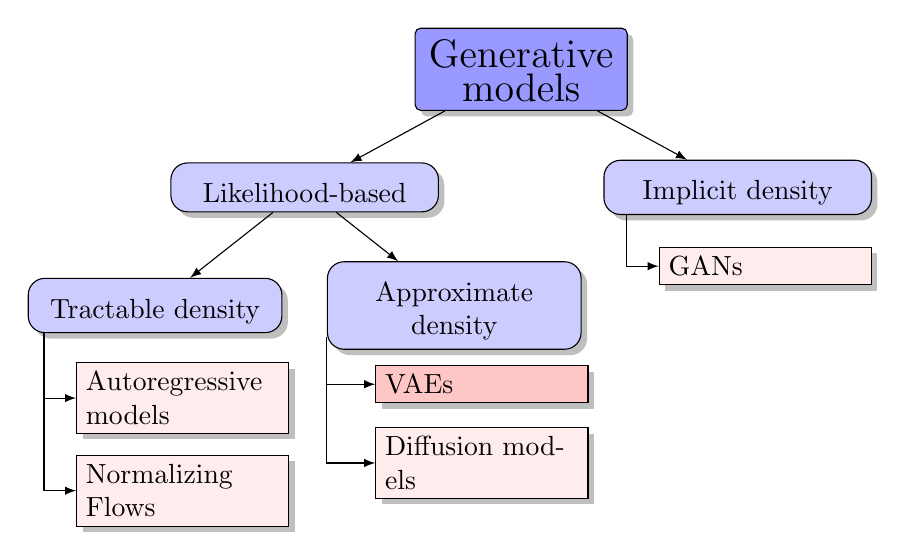
\begin{tikzpicture}[
	 	basic/.style  = {draw, text width=2cm, drop shadow, rectangle},
	 	root/.style   = {basic, rounded corners=2pt, thin, text height=1.1em, text width=7em, align=center, fill=blue!40},
	 	level 1/.style={sibling distance=55mm},
	 	level 2/.style = {basic, rounded corners=6pt, thin, align=center, fill=blue!20, text height=1.1em, text width=9em, sibling distance=38mm},
	 	level 3/.style = {basic, rounded corners=6pt, thin,align=center, fill=blue!20, text width=8.5em},
	 	level 4/.style = {basic, thin, align=left, fill=pink!30, text width=7em},
	 	level 5/.style = {basic, thin, align=left, fill=pink!90, text width=7em},
		edge from parent/.style={->,draw},
		>=latex]
		
		% root of the the initial tree, level 1
		\node[root] {\Large Generative models}
		% The first level, as children of the initial tree
		child {node[level 2] (c1) {Likelihood-based}
			child {node[level 3] (c11) {Tractable density}}
			child {node[level 3] (c12) {Approximate density}}
		}
		child {node[level 2] (c2) {Implicit density}};
				
		% The second level, relatively positioned nodes
		\begin{scope}[every node/.style={level 5}]
		\node [below of = c12, xshift=10pt] (c121) {VAEs};
		\end{scope}
		
		% The second level, relatively positioned nodes
		\begin{scope}[every node/.style={level 4}]
		\node [below of = c11, yshift=-5pt, xshift=10pt] (c111) {Autoregressive models};
		\node [below of = c111, yshift=-5pt] (c112) {Normalizing Flows};
		
		\node [below of = c121] (c122) {Diffusion models};
		\node [below of = c2, xshift=10pt] (c21) {GANs};
		
		\end{scope}
		
		
		% lines from each level 1 node to every one of its "children"
		\foreach \value in {1,2}
		\draw[->] (c11.194) |- (c11\value.west);
		
		\foreach \value in {1,2}
		\draw[->] (c12.194) |- (c12\value.west);
		
		\draw[->] (c2.194) |- (c21.west);
		
	\end{tikzpicture}
\end{frame}
%=======
\begin{frame}{Variational autoencoder (VAE)}
	\begin{block}{Final EM-algorithm}
		\begin{itemize}
			\item pick random sample $\bx_i, i \sim U[1, n]$.
			\item compute the objective:
			\vspace{-0.3cm}
			\[
				\bepsilon^* \sim r(\bepsilon); \quad \bz^* = g(\bx, \bepsilon^*, \bphi);
			\]
			\[
				\cL(\bphi, \btheta) \approx  \log p(\bx | \bz^*, \btheta) - KL(q(\bz^* | \bx, \bphi) || p(\bz^*)).
			\]
			\item compute a stochastic gradients w.r.t. $\bphi$ and $\btheta$
			\begin{align*}
				\nabla_{\bphi} \mathcal{L} (\bphi, \btheta) &\approx \nabla_{\bphi} \log p(\bx | g(\bx, \bepsilon^*, \bphi), \btheta)  - \nabla_{\bphi} \text{KL}(q(\bz | \bx, \bphi) || p(\bz)); \\
				\nabla_{\btheta} \mathcal{L} (\bphi, \btheta) &\approx \nabla_{\btheta} \log p(\bx|\bz^*, \btheta).
			\end{align*}
			\item update $\btheta, \bphi$ according to the selected optimization method (SGD, Adam, RMSProp):
			\begin{align*}
				\bphi &:= \bphi + \eta \nabla_{\bphi} \mathcal{L}(\bphi, \btheta), \\
				\btheta &:= \btheta + \eta \nabla_{\btheta} \mathcal{L}(\bphi, \btheta).
			\end{align*}
		\end{itemize}
	\end{block}
\end{frame}
%=======
\begin{frame}{Variational autoencoder (VAE)}
	\begin{minipage}[t]{0.55\columnwidth}
	    \begin{itemize}
	    \item VAE learns stochastic mapping between $\bx$-space, from complicated distribution $\pi(\bx)$, and a latent $\bz$-space, with simple distribution. 
	    \item The generative model learns a joint distribution $p(\bx, \bz | \btheta) = p(\bz) p(\bx |\bz, \btheta)$, with a prior distribution $p(\bz)$, and a stochastic decoder $p(\bx|\bz, \btheta)$. 
	    \item The stochastic encoder $q(\bz|\bx, \bphi)$ (inference model), approximates the true but intractable posterior $p(\bz|\bx, \btheta)$ of the generative model.
	    \end{itemize}
	\end{minipage}%
	\begin{minipage}[t]{0.45\columnwidth}
		\begin{figure}[h]
			\centering
			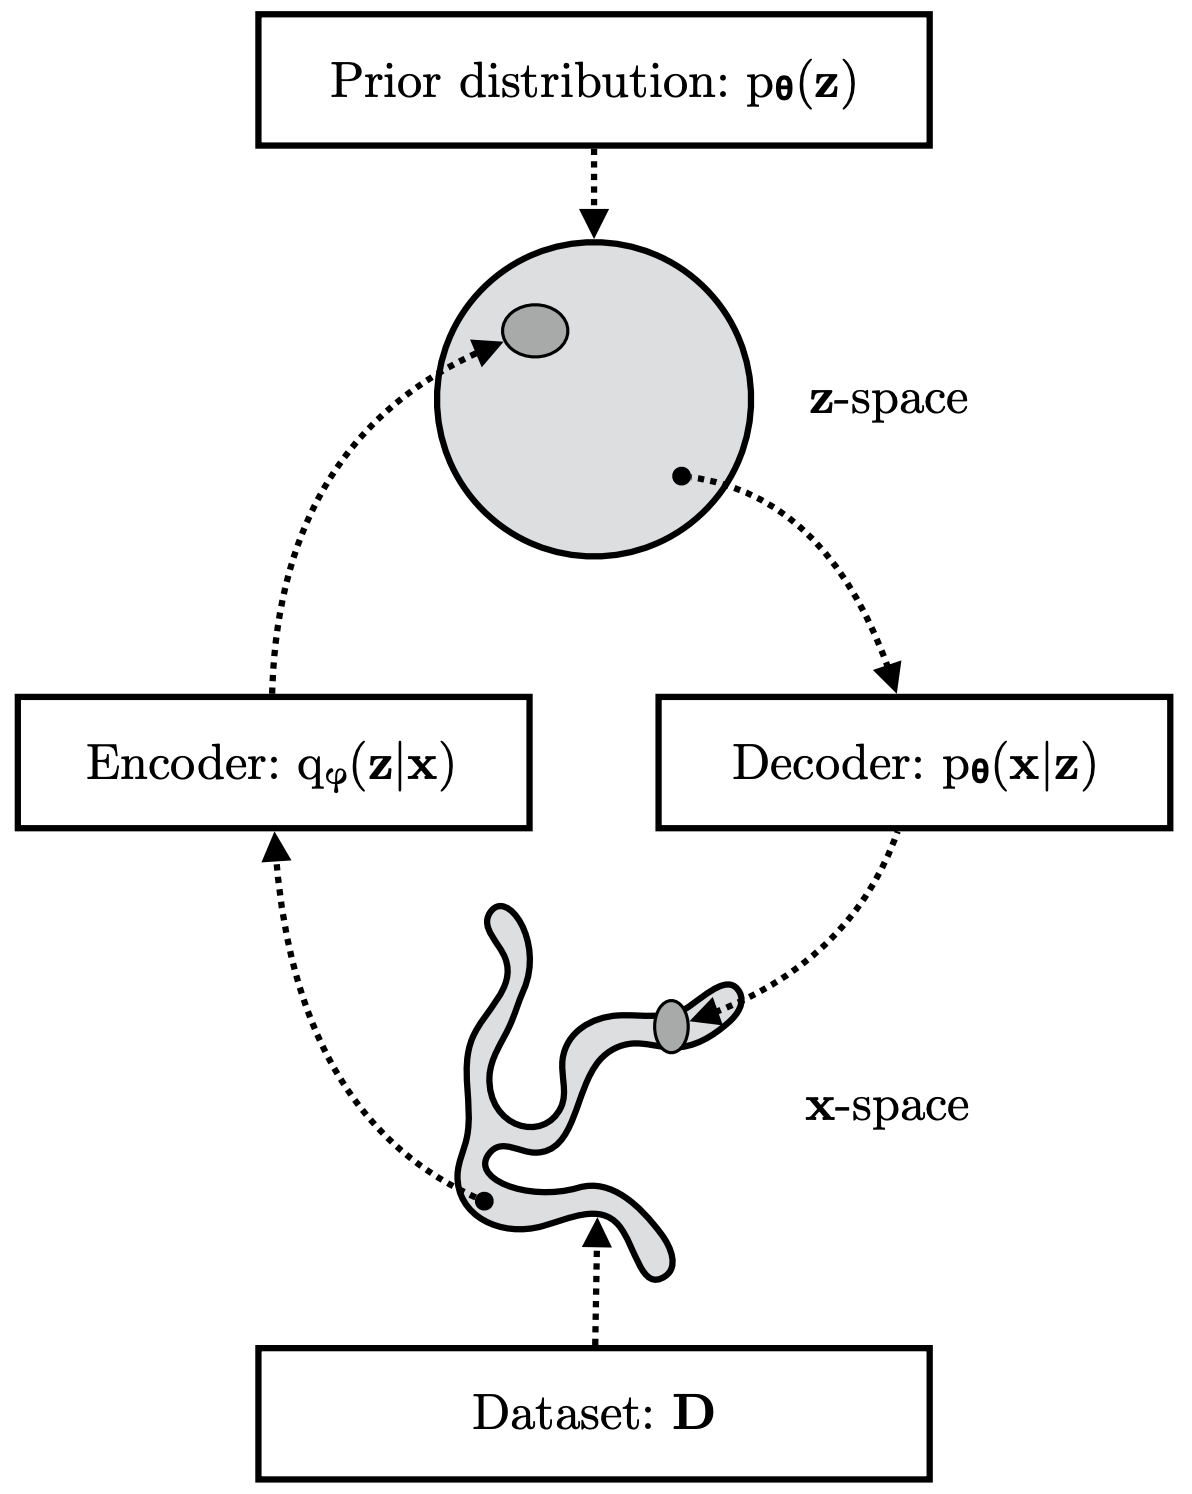
\includegraphics[width=\linewidth]{figs/vae_scheme}
		\end{figure}
	\end{minipage}
	
	\myfootnotewithlink{https://arxiv.org/abs/1906.02691}{Kingma D. P., Welling M. An introduction to variational autoencoders, 2019}
\end{frame}
%=======
\begin{frame}{Variational Autoencoder}
	\[
		 \mathcal{L} (\bphi, \btheta)  = \mathbb{E}_{q(\bz | \bx, \bphi)} \left[\log p(\bx | \bz, \btheta) - \log \frac{q(\bz | \bx, \bphi)}{p(\bz)} \right] \rightarrow \max_{\bphi, \btheta}.
	\]	
	\vspace{-0.3cm}
	\begin{figure}[h]
		\centering
		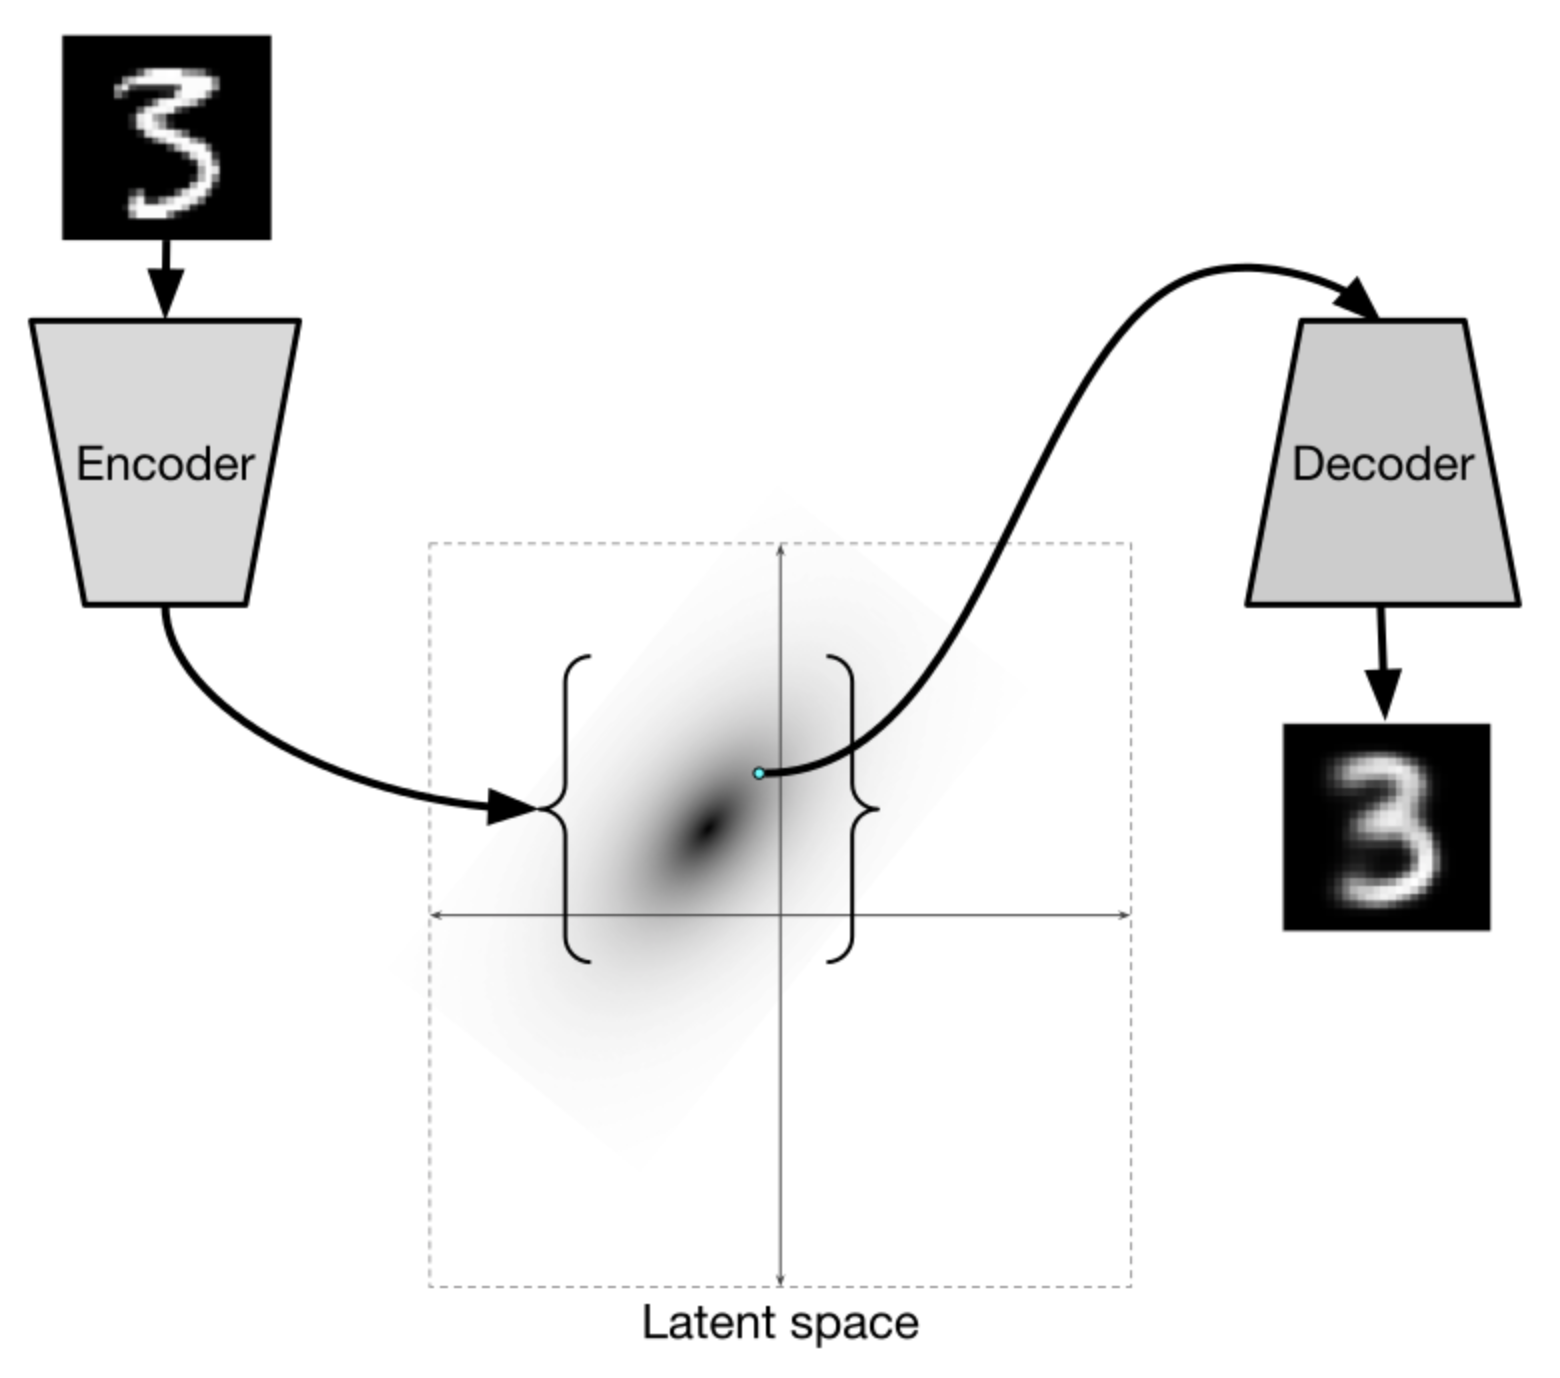
\includegraphics[width=.65\linewidth]{figs/VAE.png}
	\end{figure}
	\myfootnotewithlink{http://ijdykeman.github.io/ml/2016/12/21/cvae.html}{image credit: http://ijdykeman.github.io/ml/2016/12/21/cvae.html}
\end{frame}
%=======
\begin{frame}{Variational autoencoder (VAE)}
	\begin{itemize}
		\item Encoder $q(\bz | \bx, \bphi) = \text{NN}_e(\bx, \bphi)$ outputs $\bmu_{\bphi}(\bx)$ and $\bsigma_{\bphi}(\bx)$.
		\item Decoder $p(\bx | \bz, \btheta) = \text{NN}_d(\bz, \btheta)$ outputs parameters of the sample distribution.
	\end{itemize}
	\begin{figure}[h]
		\centering
		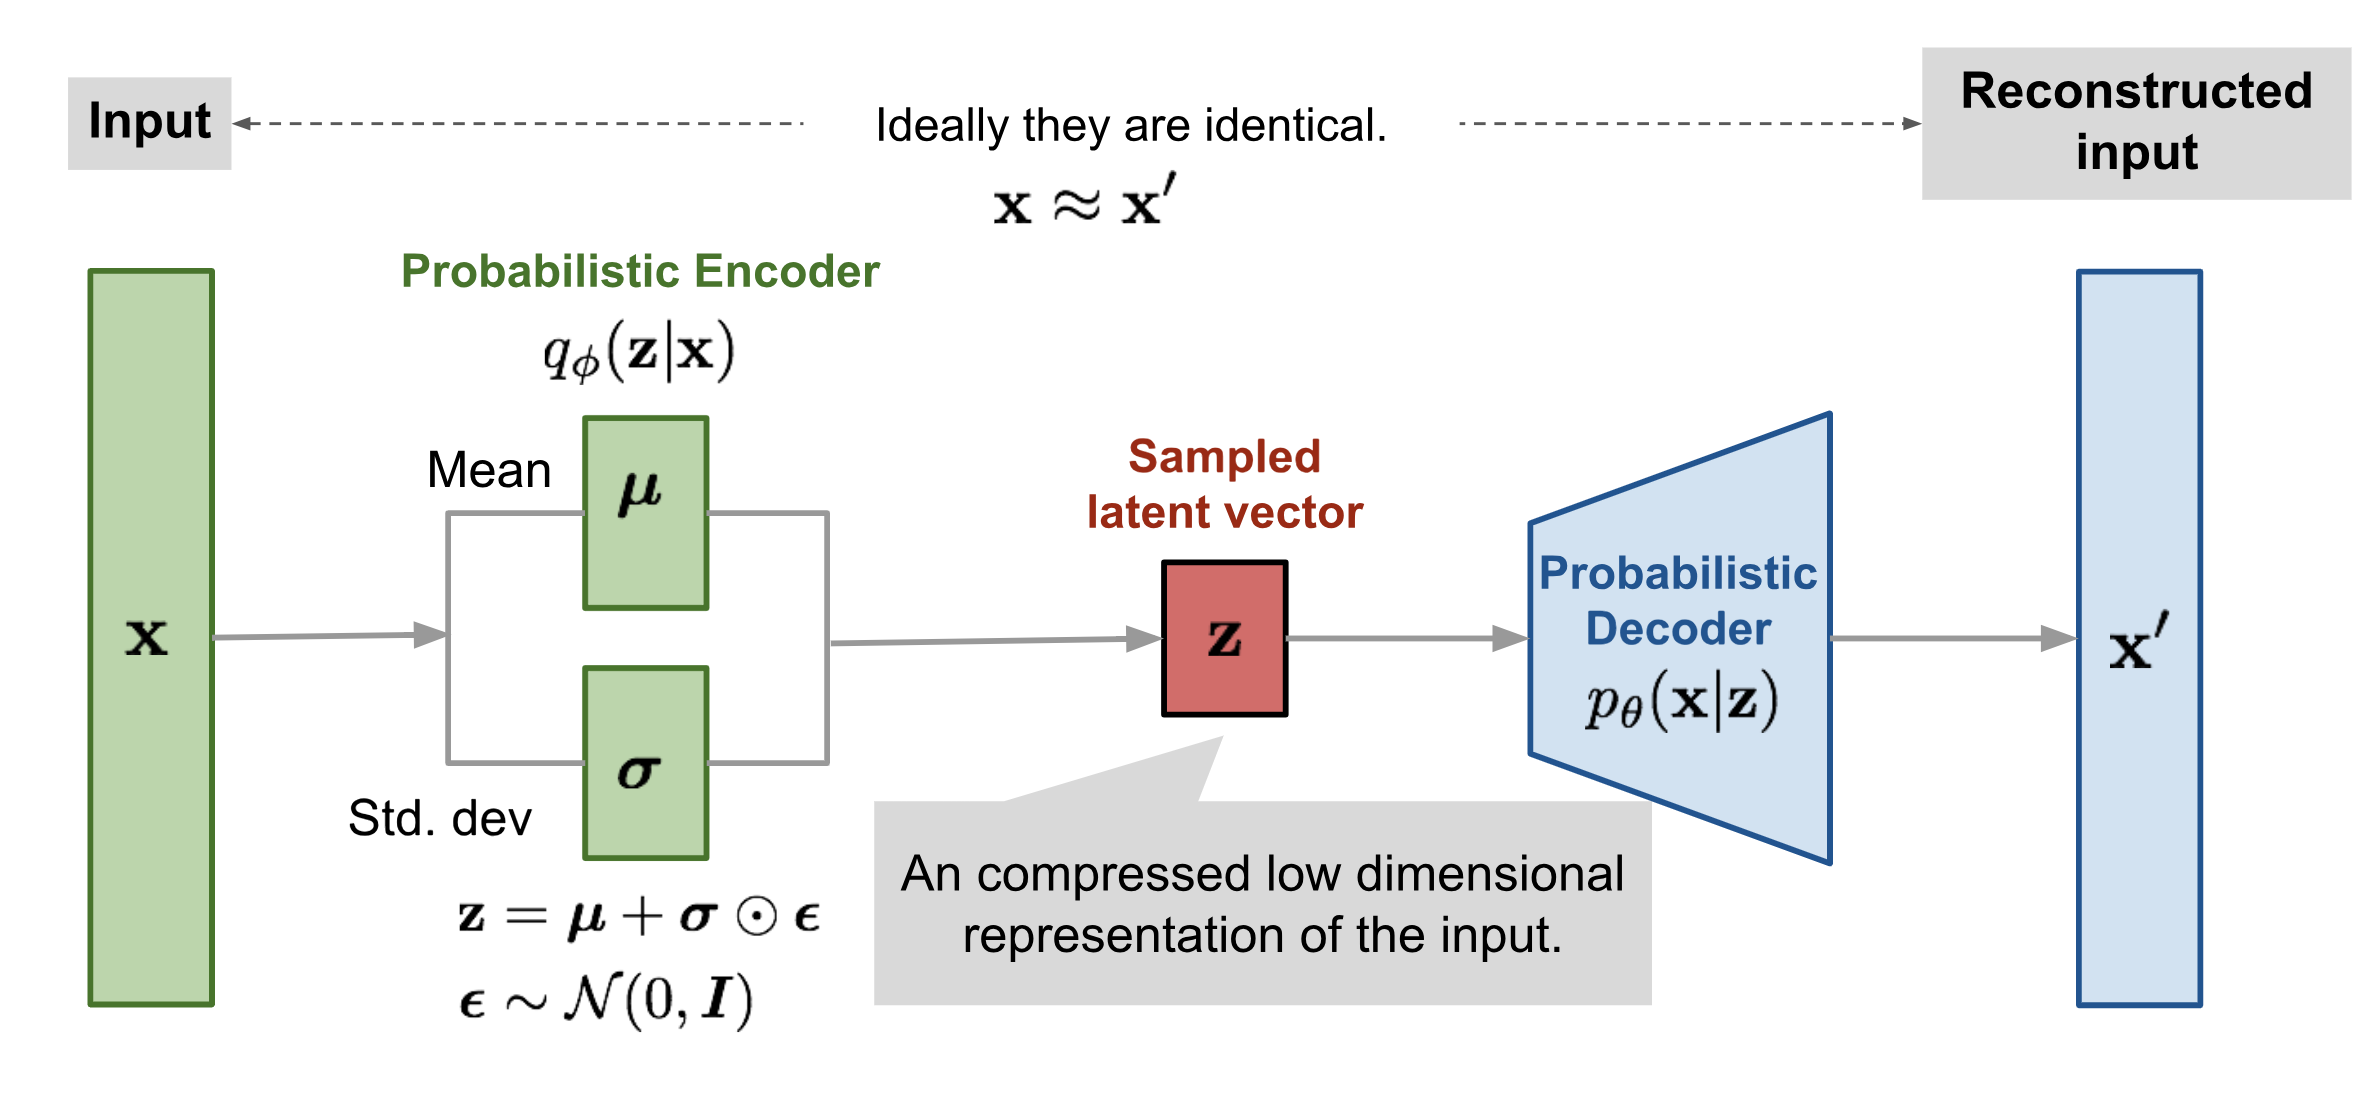
\includegraphics[width=\linewidth]{figs/vae-gaussian.png}
	\end{figure}
	
	\myfootnotewithlink{https://lilianweng.github.io/lil-log/2018/08/12/from-autoencoder-to-beta-vae.html}{image credit: https://lilianweng.github.io/lil-log/2018/08/12/from-autoencoder-to-beta-vae.html}
\end{frame}
%=======
\begin{frame}{VAE limitations}
	\begin{itemize}
		\item Poor generative distribution (decoder)
		\[
			p(\bx | \bz, \btheta) = \mathcal{N}(\bx| \bmu_{\btheta}(\bz), \bsigma^2_{\btheta}(\bz)) \quad \text{or } = \text{Softmax}(\bpi_{\btheta}(\bz)).
		\]
		\item Loose lower bound
		\[
			\log p(\bx | \btheta) - \mathcal{L}(q, \btheta) = (?).
		\]
		\item Poor prior distribution
		\[
			p(\bz) = \mathcal{N}(0, \mathbf{I}).
		\]
		\item Poor variational posterior distribution (encoder)
		\[
			q(\bz | \bx, \bphi) = \mathcal{N}(\bz| \bmu_{\bphi}(\bx), \bsigma^2_{\bphi}(\bx)).
		\]
	\end{itemize}
\end{frame}
%=======
\begin{frame}{VAE as Bayesian model}
	\begin{block}{Posterior distribution}
		\vspace{-0.2cm}
		\[
			p(\btheta | \bX) = \frac{p(\bX | \btheta) p(\btheta)}{p(\bX)}
		\]
		\vspace{-0.5cm}
	\end{block}
	\begin{block}{ELBO}
		\vspace{-0.5cm}
		\begin{align*}
			 \log p(\btheta | \bX) &= \log p(\bX | \btheta) + \log p(\btheta) - \log p(\bX) \\
			 &= \cL(q, \btheta) + KL(q || p) + \log p(\btheta) - \log p(\bX) \\
			 &\geq \left[ \cL(q, \btheta) + \log p(\btheta) \right] - \log p(\bX) .
		\end{align*}
		\vspace{-0.7cm}
	\end{block}
	\begin{block}{EM-algorithm}
		\begin{itemize}
			\item E-step
				\vspace{-0.2cm}
				\[
					q(\bz) = \argmax_q \mathcal{L} (q, \btheta^*) = \argmin_q KL(q || p) =
				 p(\bz| \bx, \btheta^*);
				\]
				\vspace{-0.5cm}
			\item M-step
				\[
					\btheta^* = \argmax_{\btheta} \left[ \mathcal{L} (q, \btheta) + \log p(\btheta) \right].
				\]
		\end{itemize}
	\end{block}
\end{frame}
%=======
\section{Posterior collapse and decoder weakening techniques}
%=======
\begin{frame}{VAE limitations}
	\begin{itemize}
		\item \textbf{Poor generative distribution (decoder)}
		\[
			p(\bx | \bz, \btheta) = \mathcal{N}(\bx| \bmu_{\btheta}(\bz), \bsigma^2_{\btheta}(\bz)) \quad \text{or } = \text{Softmax}(\bpi_{\btheta}(\bz)).
		\]
		\item Loose lower bound
		\[
			\log p(\bx | \btheta) - \mathcal{L}(q, \btheta) = (?).
		\]
		\item Poor prior distribution
		\[
			p(\bz) = \mathcal{N}(0, \mathbf{I}).
		\]
		\item Poor variational posterior distribution (encoder)
		\[
			q(\bz | \bx, \bphi) = \mathcal{N}(\bz| \bmu_{\bphi}(\bx), \bsigma^2_{\bphi}(\bx)).
		\]
	\end{itemize}
\end{frame}
%=======
\begin{frame}{Posterior collapse}
	\begin{block}{LVM}
		\vspace{-0.3cm}
		\[
   			p(\bx | \btheta) = \int p(\bx, \bz | \btheta) d \bz = \int p(\bx | \bz, \btheta) p(\bz) d \bz 
		\]
		\vspace{-0.5cm}
	\end{block}
	\begin{block}{ELBO objective}
		\vspace{-0.3cm}
		\[
			\mathcal{L}(\bphi, \btheta) = \left[ \mathbb{E}_{q(\bz | \bx, \bphi)} \log p(\bx | \bz, \btheta) - KL(q(\bz | \bx, \bphi) || p(\bz)) \right].
		\]
	\end{block}
	\begin{itemize}
		\item More powerful $p(\bx | \bz, \btheta)$ leads to more powerful generative model $p(\bx | \btheta)$.
		\item If the decoder $p(\bx | \bz, \btheta)$ is too powerful (it could  model $p(\bx | \btheta)$), then the latent variables $\bz$ becomes irrelevant. ELBO avoids paying any cost $KL(q(\bz| \bx, \bphi)||p(\bz))$ ($q(\bz| \bx, \bphi) \approx p(\bz)$), the variational posterior $q(\bz | \bx, \bphi)$ will not carry any information about $\bx$ .
	\end{itemize}
	How to make the generative model $p(\bx | \bz, \btheta)$ more powerful?
\end{frame}
%=======
\begin{frame}{PixelVAE}
	\begin{block}{Autoregressive decoder}
		\vspace{-0.3cm}
		\[
		p(\bx | \bz , \btheta) = \prod_{j=1}^m p(x_j | \bx_{1:j - 1}, \bz , \btheta)
		\]
		\vspace{-0.3cm}
	\end{block}
	\begin{itemize}
		\item Global structure is captured by latent variables.
		\item Local statistics are captured by limited receptive field autoregressive model.
	\end{itemize}
	\vspace{-0.1cm}
	\begin{block}{MNIST results}
		\vspace{-0.3cm}
		\begin{figure}
		    \centering
		    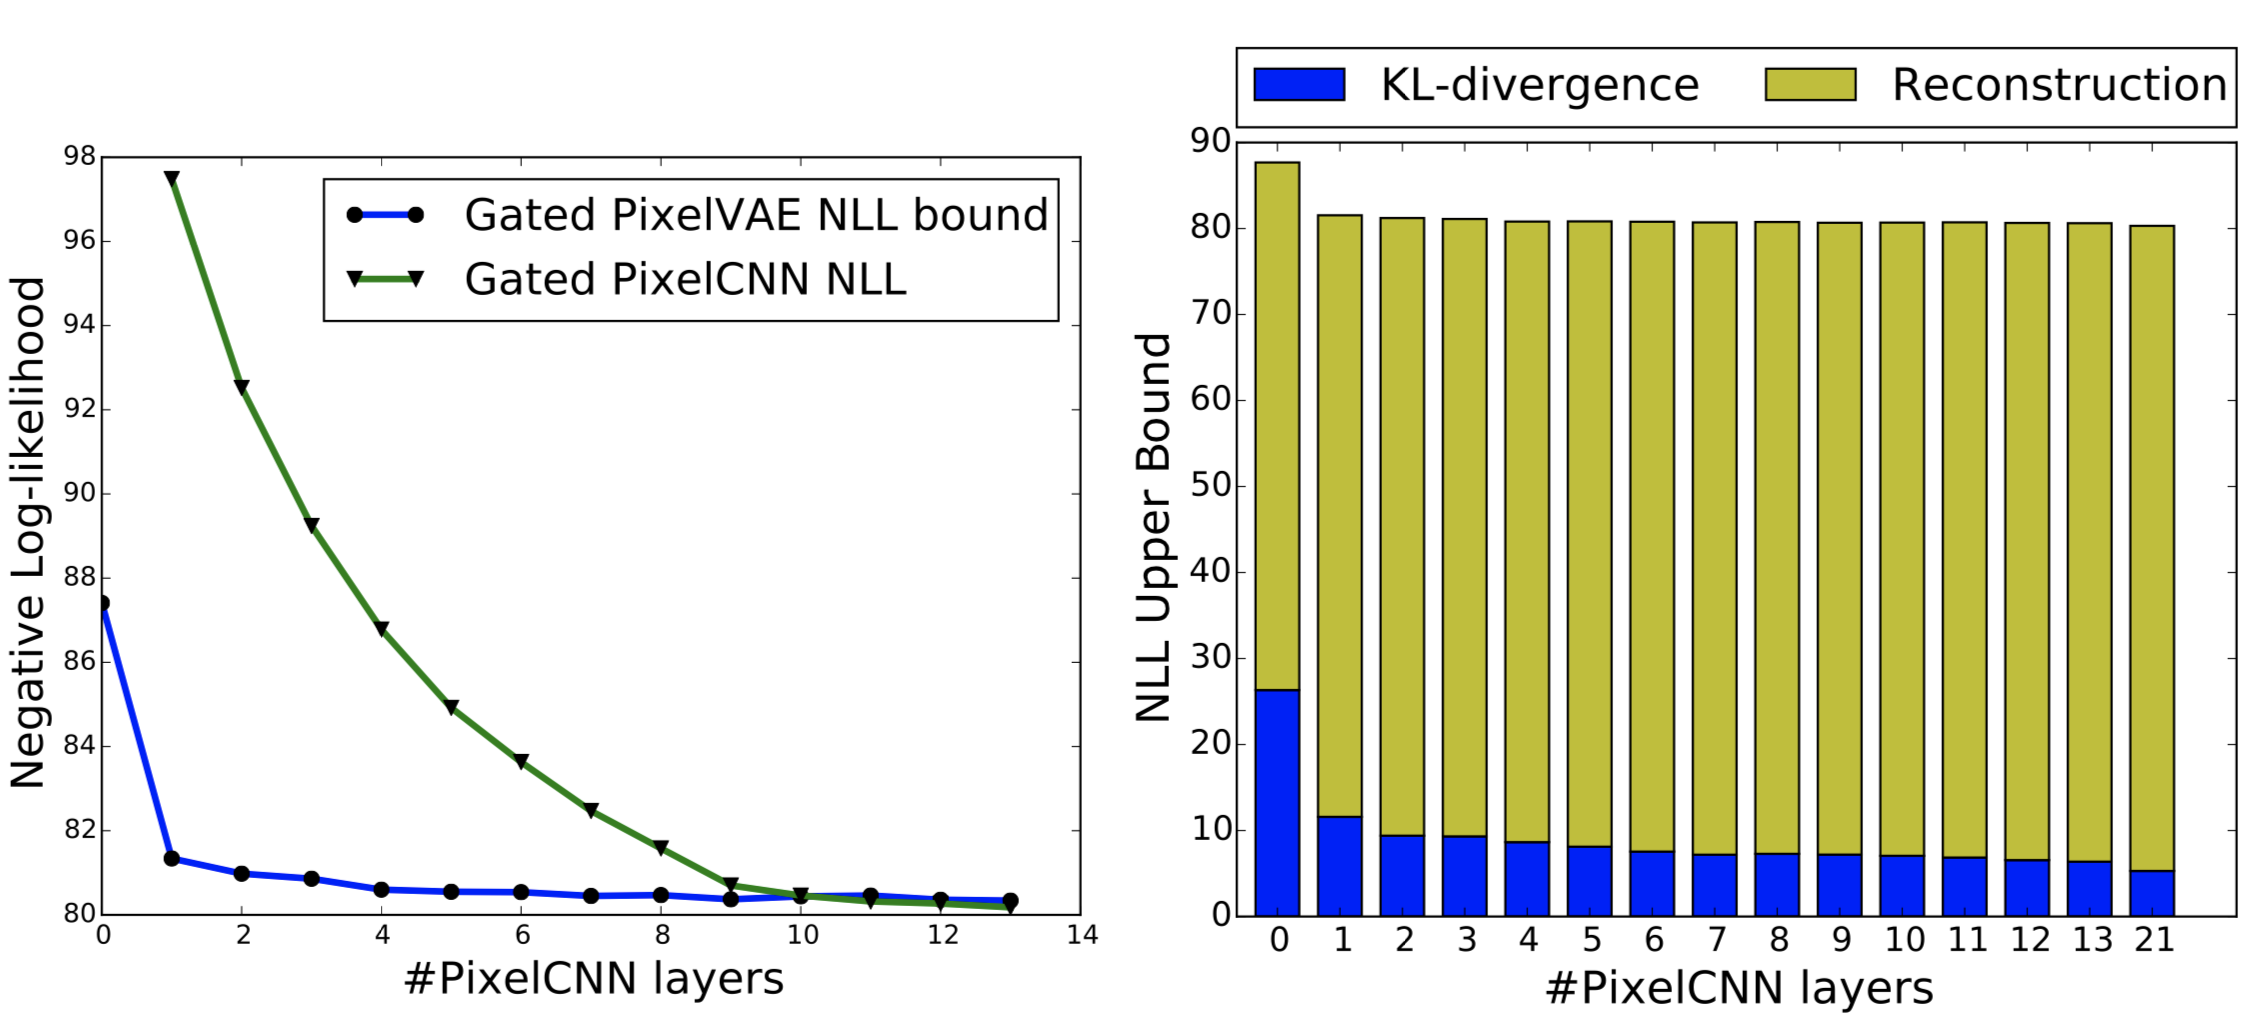
\includegraphics[width=0.75\linewidth]{figs/PixelVAE_2.png}
		\end{figure}
	\end{block}
		
	\myfootnotewithlink{https://arxiv.org/abs/1611.05013}{Gulrajani I. et al. PixelVAE: A Latent Variable Model for Natural Images, 2016}
\end{frame}
%=======
\begin{frame}{Decoder weakening techniques}
	\vspace{-0.3cm}
	\begin{itemize}
		\item Powerful decoder $p(\bx | \bz, \btheta)$ makes the model expressive, but posterior collapse is possible.
		\item PixelVAE model uses the autoregressive PixelCNN model with small number of layers to limit receptive field.
	\end{itemize}
	How to force the model encode information about $\bx$ into $\bz$?
	\begin{block}{KL annealing}
		\vspace{-0.7cm}
		\[
		    \mathcal{L}(\bphi, \btheta, \beta) = \mathbb{E}_{q(\bz | \bx, \bphi)} \log p(\bx | \bz, \btheta) - \beta \cdot KL (q(\bz | \bx, \bphi) || p(\bz))
		\]
		\vspace{-0.7cm} \\
		Start training with $\beta = 0$, increase it until $\beta = 1$ during training.
	\end{block}
	\begin{block}{Free bits}
		\vspace{-0.7cm}
		\[
		    \mathcal{L}(\bphi, \btheta, \lambda) = \mathbb{E}_{q(\bz | \bx, \bphi)} \log p(\bx | \bz, \btheta) - \max(\lambda, KL (q(\bz | \bx, \bphi) || p(\bz))).
		\]
		\vspace{-0.7cm} \\
		It ensures the use of less than $\lambda$ bits of information and results in $KL (q(\bz | \bx, \bphi) || p(\bz)) \geq \lambda$.
	\end{block}
	\myfootnote{\href{https://arxiv.org/abs/1511.06349}{Bowman S. R. et al. Generating Sentences from a Continuous Space, 2015} \\
	\href{https://arxiv.org/abs/1606.04934}{Kingma D. P. et al. Improving Variational Inference with Inverse Autoregressive Flow, 2016}}
\end{frame}
%=======
\section{Tighter variational bound}
%=======
\begin{frame}{VAE limitations}
	\begin{itemize}
		\item Poor generative distribution (decoder)
		\[
			p(\bx | \bz, \btheta) = \mathcal{N}(\bx| \bmu_{\btheta}(\bz), \bsigma^2_{\btheta}(\bz)) \quad \text{or } = \text{Softmax}(\bpi_{\btheta}(\bz)).
		\]
		\item \textbf{Loose lower bound}
		\[
			\log p(\bx | \btheta) - \mathcal{L}(q, \btheta) = (?).
		\]
		\item Poor prior distribution
		\[
			p(\bz) = \mathcal{N}(0, \mathbf{I}).
		\]
		\item Poor variational posterior distribution (encoder)
		\[
			q(\bz | \bx, \bphi) = \mathcal{N}(\bz| \bmu_{\bphi}(\bx), \bsigma^2_{\bphi}(\bx)).
		\]
	\end{itemize}
\end{frame}
%=======
\begin{frame}{Importance sampling}
	\begin{block}{LVM}
		\vspace{-0.5cm}
		\begin{align*}
			p(\bx | \btheta) &= \int p(\bx, \bz | \btheta) d\bz = \int \left[\frac{p(\bx, \bz | \btheta)}{q(\bz | \bx, \bphi)} \right] q(\bz | \bx, \bphi) d\bz \\
			&= \int f(\bx, \bz) q(\bz | \bx, \bphi) d\bz = \mathbb{E}_{\bz \sim q(\bz | \bx, \bphi)} f(\bx, \bz)
		\end{align*}
	\end{block}
	Here $f(\bx, \bz) = \frac{p(\bx, \bz | \btheta)}{q(\bz | \bx, \bphi)}$.
	\begin{block}{ELBO: derivation 1}
		\vspace{-0.5cm}
		\begin{multline*}
			\log p(\bx | \btheta) = \log \mathbb{E}_{\bz \sim q(\bz | \bx, \bphi)} f(\bx, \bz)
			\geq \mathbb{E}_{\bz \sim q(\bz | \bx, \bphi)} \log f(\bx, \bz) = \\
			= \mathbb{E}_{\bz \sim q(\bz | \bx, \bphi)} \log \frac{p(\bx, \bz | \btheta)}{q(\bz | \bx, \bphi)} = \mathcal{L}(q, \btheta).
		\end{multline*}
	\end{block}
	Could we choose better $f(\bx, \bz)$? 
\end{frame}
%=======
\begin{frame}{Importance Weighted Autoencoders (IWAE)}
		\[
			p(\bx | \btheta) = \int \left[\frac{p(\bx, \bz | \btheta)}{q(\bz | \bx, \bphi)} \right] q(\bz | \bx, \bphi) d\bz = \mathbb{E}_{\bz \sim q(\bz | \bx, \bphi)} f(\bx, \bz)
		\]
	Let define
	\[
	f(\bx, \bz_1, \dots, \bz_K) = \frac{1}{K} \sum_{k=1}^K \frac{p(\bx, \bz_k | \btheta)}{q(\bz_k | \bx, \bphi)}
	\]
	\[
		\mathbb{E}_{\bz_1, \dots, \bz_K \sim q(\bz | \bx, \bphi)} f(\bx, \bz_1, \dots, \bz_K) = p(\bx | \btheta)
	\]
	\vspace{-0.3cm}
	\begin{block}{ELBO}
		\vspace{-0.5cm}
		\begin{multline*}
			\log p(\bx | \btheta) = \log \mathbb{E}_{\bz_1, \dots, \bz_K \sim q(\bz | \bx)} f(\bx, \bz, \dots, \bz_K) \geq \\
			\geq \mathbb{E}_{\bz_1, \dots, \bz_K \sim q(\bz | \bx, \bphi)} \log f(\bx, \bz, \dots, \bz_K) = \\
			= \mathbb{E}_{\bz_1, \dots, \bz_K \sim q(\bz | \bx, \bphi)} \log \left[\frac{1}{K} \sum_{k=1}^K\frac{p(\bx, \bz_k | \btheta)}{q(\bz_k | \bx, \bphi)} \right] = \mathcal{L}_K(q, \btheta).
		\end{multline*}
	\end{block}
	\myfootnotewithlink{https://arxiv.org/abs/1509.00519}{Burda Y., Grosse R., Salakhutdinov R. Importance Weighted Autoencoders, 2015}
\end{frame}
%=======
\begin{frame}{Importance Weighted Autoencoders (IWAE)}
	\begin{block}{VAE objective}
		\vspace{-0.2cm}
		\[
		\log p(\bx | \btheta) \geq \mathcal{L} (q, \btheta)  = \mathbb{E}_{q(\bz | \bx, \bphi)} \log \frac{p(\bx, \bz | \btheta)}{q(\bz| \bx, \bphi)} \rightarrow \max_{q, \btheta}
		\]
		\[
		\mathcal{L} (q, \btheta)  = \mathbb{E}_{\bz_1, \dots, \bz_K \sim q(\bz | \bx, \bphi)} \left( \frac{1}{K} \sum_{k=1}^K \log \frac{p(\bx, \bz_k | \btheta)}{q(\bz_k| \bx, \bphi)} \right) \rightarrow \max_{q, \btheta}.
		\]
		\vspace{-0.2cm}
	\end{block}
	\begin{block}{IWAE objective}
		\vspace{-0.2cm}
		\[
			\mathcal{L}_K (q, \btheta)  = \mathbb{E}_{\bz_1, \dots, \bz_K \sim q(\bz | \bx, \bphi)} \log \left( \frac{1}{K}\sum_{k=1}^K\frac{p(\bx, \bz_k | \btheta)}{q(\bz_k| \bx, \bphi)} \right) \rightarrow \max_{q, \btheta}.
		\]
	\end{block}
	If $K=1$, these objectives coincide.

	\myfootnotewithlink{https://arxiv.org/abs/1509.00519}{Burda Y., Grosse R., Salakhutdinov R. Importance Weighted Autoencoders, 2015}
\end{frame}
%=======
\begin{frame}{Importance Weighted Autoencoders (IWAE)}
	\begin{block}{Theorem}
		\begin{enumerate}
			\item $\log p(\bx | \btheta) \geq \mathcal{L}_K (q, \btheta) \geq \mathcal{L}_M (q, \btheta), \quad \text{for } K \geq M$;
			\item $\log p(\bx | \btheta) = \lim_{K \rightarrow \infty} \mathcal{L}_K (q, \btheta)$ if $\frac{p(\bx, \bz | \btheta)}{q(\bz | \bx, \bphi)}$ is bounded.
		\end{enumerate}
		\vspace{-0.2cm}
	\end{block}
	If $K > 1$ the bound could be tighter.
	\begin{align*}
		\mathcal{L} (q, \btheta) &= \mathbb{E}_{q(\bz | \bx, \bphi)} \log \frac{p(\bx, \bz | \btheta)}{q(\bz| \bx, \bphi)}; \\
		\mathcal{L}_K (q, \btheta) &= \mathbb{E}_{\bz_1, \dots, \bz_K \sim q(\bz | \bx, \bphi)} \log \left( \frac{1}{K}\sum_{k=1}^K\frac{p(\bx, \bz_k | \btheta)}{q(\bz_k| \bx, \bphi)} \right).
	\end{align*}
	\vspace{-0.2cm}
	\begin{itemize}
		\item $\mathcal{L}_1(q, \btheta) = \mathcal{L}(q, \btheta)$;
		\item $\mathcal{L}_{\infty}(q, \btheta) = \log p(\bx | \btheta)$.
		\item Which $q^*(\bz | \bx, \bphi)$ gives $\mathcal{L}(q^*, \btheta) = \log p(\bx | \btheta)$? 
	\end{itemize}

	\myfootnotewithlink{https://arxiv.org/abs/1509.00519}{Burda Y., Grosse R., Salakhutdinov R. Importance Weighted Autoencoders, 2015}
\end{frame}
%=======
\begin{frame}{Importance Weighted Autoencoders (IWAE)}
	\begin{block}{Objective}
		\vspace{-0.5cm}
		\[
		\mathcal{L}_K (q, \btheta)  = \mathbb{E}_{\bz_1, \dots, \bz_K \sim q(\bz | \bx, \bphi)} \log \left( \frac{1}{K}\sum_{k=1}^K\frac{p(\bx, \bz_k | \btheta)}{q(\bz_k| \bx, \bphi)} \right) \rightarrow \max_{\bphi, \btheta}.
		\]
		\vspace{-0.3cm}
	\end{block}
	\begin{block}{Gradient}
		\vspace{-0.3cm}
		\[
		\Delta_K = \nabla_{\btheta, \bphi} \log \left( \frac{1}{K}\sum_{k=1}^K\frac{p(\bx, \bz_k | \btheta)}{q(\bz_k| \bx, \bphi)} \right), \quad \bz_k \sim q(\bz | \bx, \bphi).
		\]
		\vspace{-0.3cm}
	\end{block}
	\begin{block}{Theorem}
		\vspace{-0.4cm}
		\[
			\text{SNR}_K = \frac{\bbE [\Delta_K]}{\sigma(\Delta_K)}; \quad
			\text{SNR}_K(\btheta) = O(\sqrt{K}); \quad 
			\text{SNR}_K(\bphi) = O\left(\sqrt{\frac{1}{K}}\right).
		\]
		Hence, increasing $K$ vanishes gradient signal of inference network $q(\bz | \bx, \bphi)$.
	\end{block}

	\myfootnotewithlink{https://arxiv.org/abs/1802.04537}{Rainforth T. et al. Tighter variational bounds are not necessarily better, 2018}
\end{frame}
%=======
\begin{frame}{Importance Weighted Autoencoders (IWAE)}
	\begin{block}{Theorem}
		\vspace{-0.5cm}
		\[
			\text{SNR}_K = \frac{\bbE [\Delta_K]}{\sigma(\Delta_K)}; \quad
			\text{SNR}_K(\btheta) = O(\sqrt{K}); \quad 
			\text{SNR}_K(\bphi) = O\left(\sqrt{\frac{1}{K}}\right).
		\]
		\vspace{-0.8cm}
	\end{block}
		\begin{minipage}[t]{0.5\columnwidth}
			\begin{figure}[h]
				\centering
				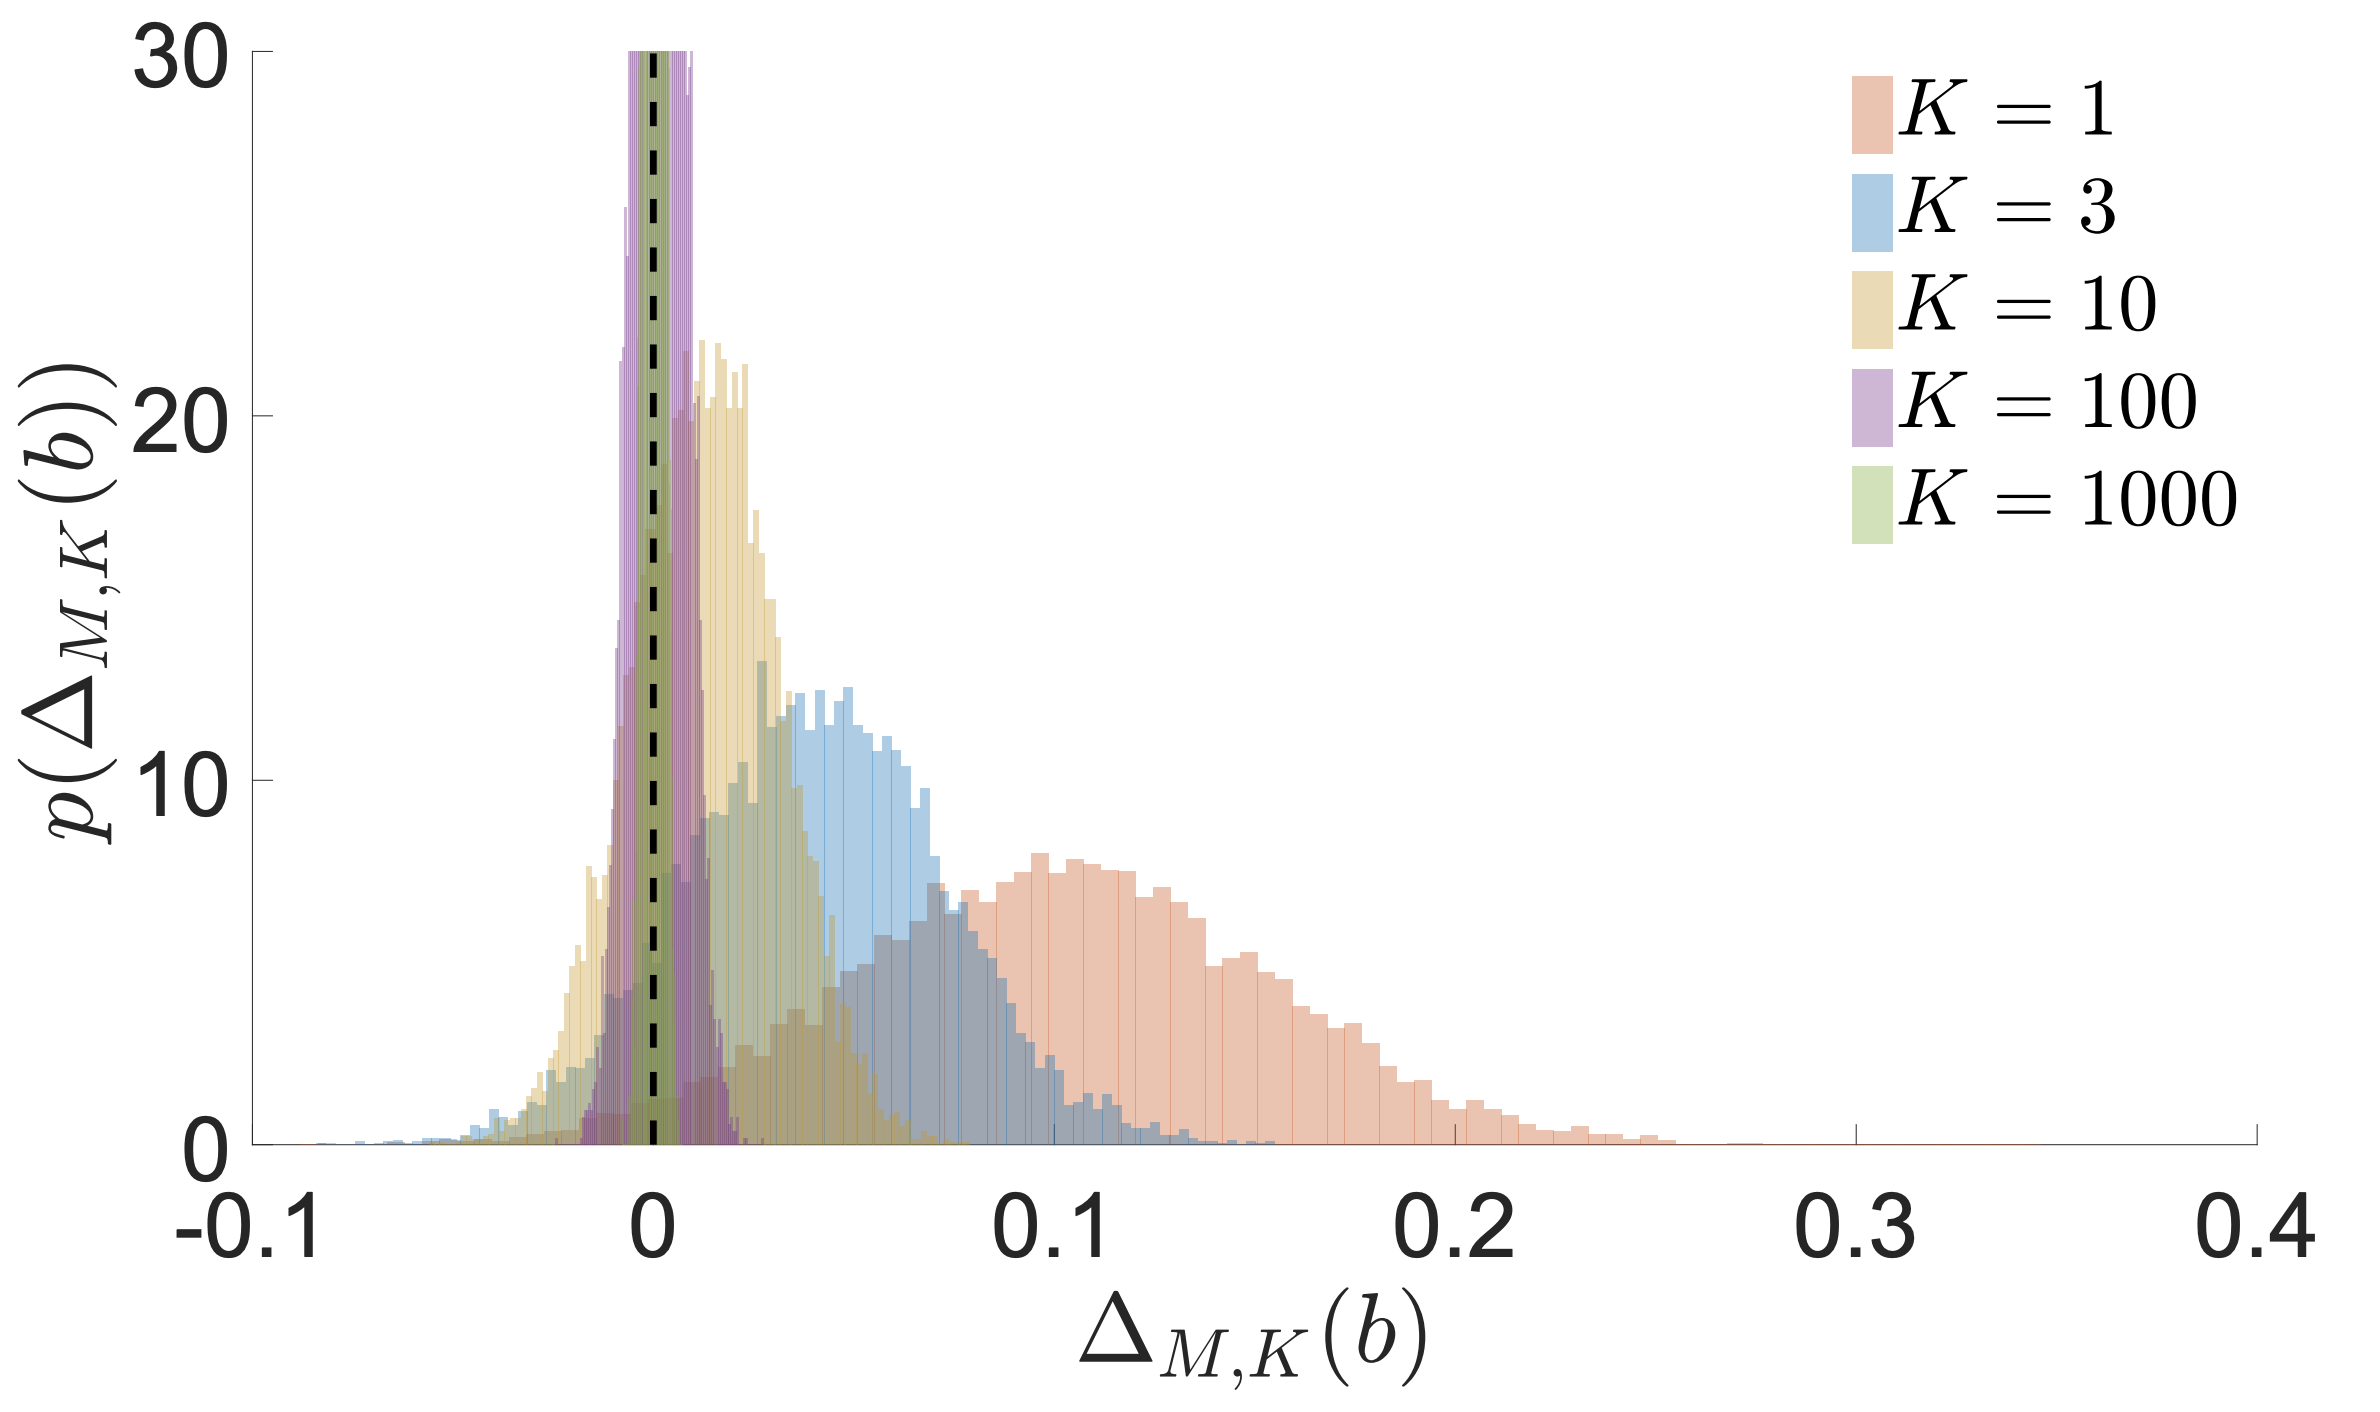
\includegraphics[width=1.\linewidth]{figs/IWAE_SNR_1.png}
			\end{figure}
		\end{minipage}%
		\begin{minipage}[t]{0.5\columnwidth}
			\begin{figure}[h]
				\centering
				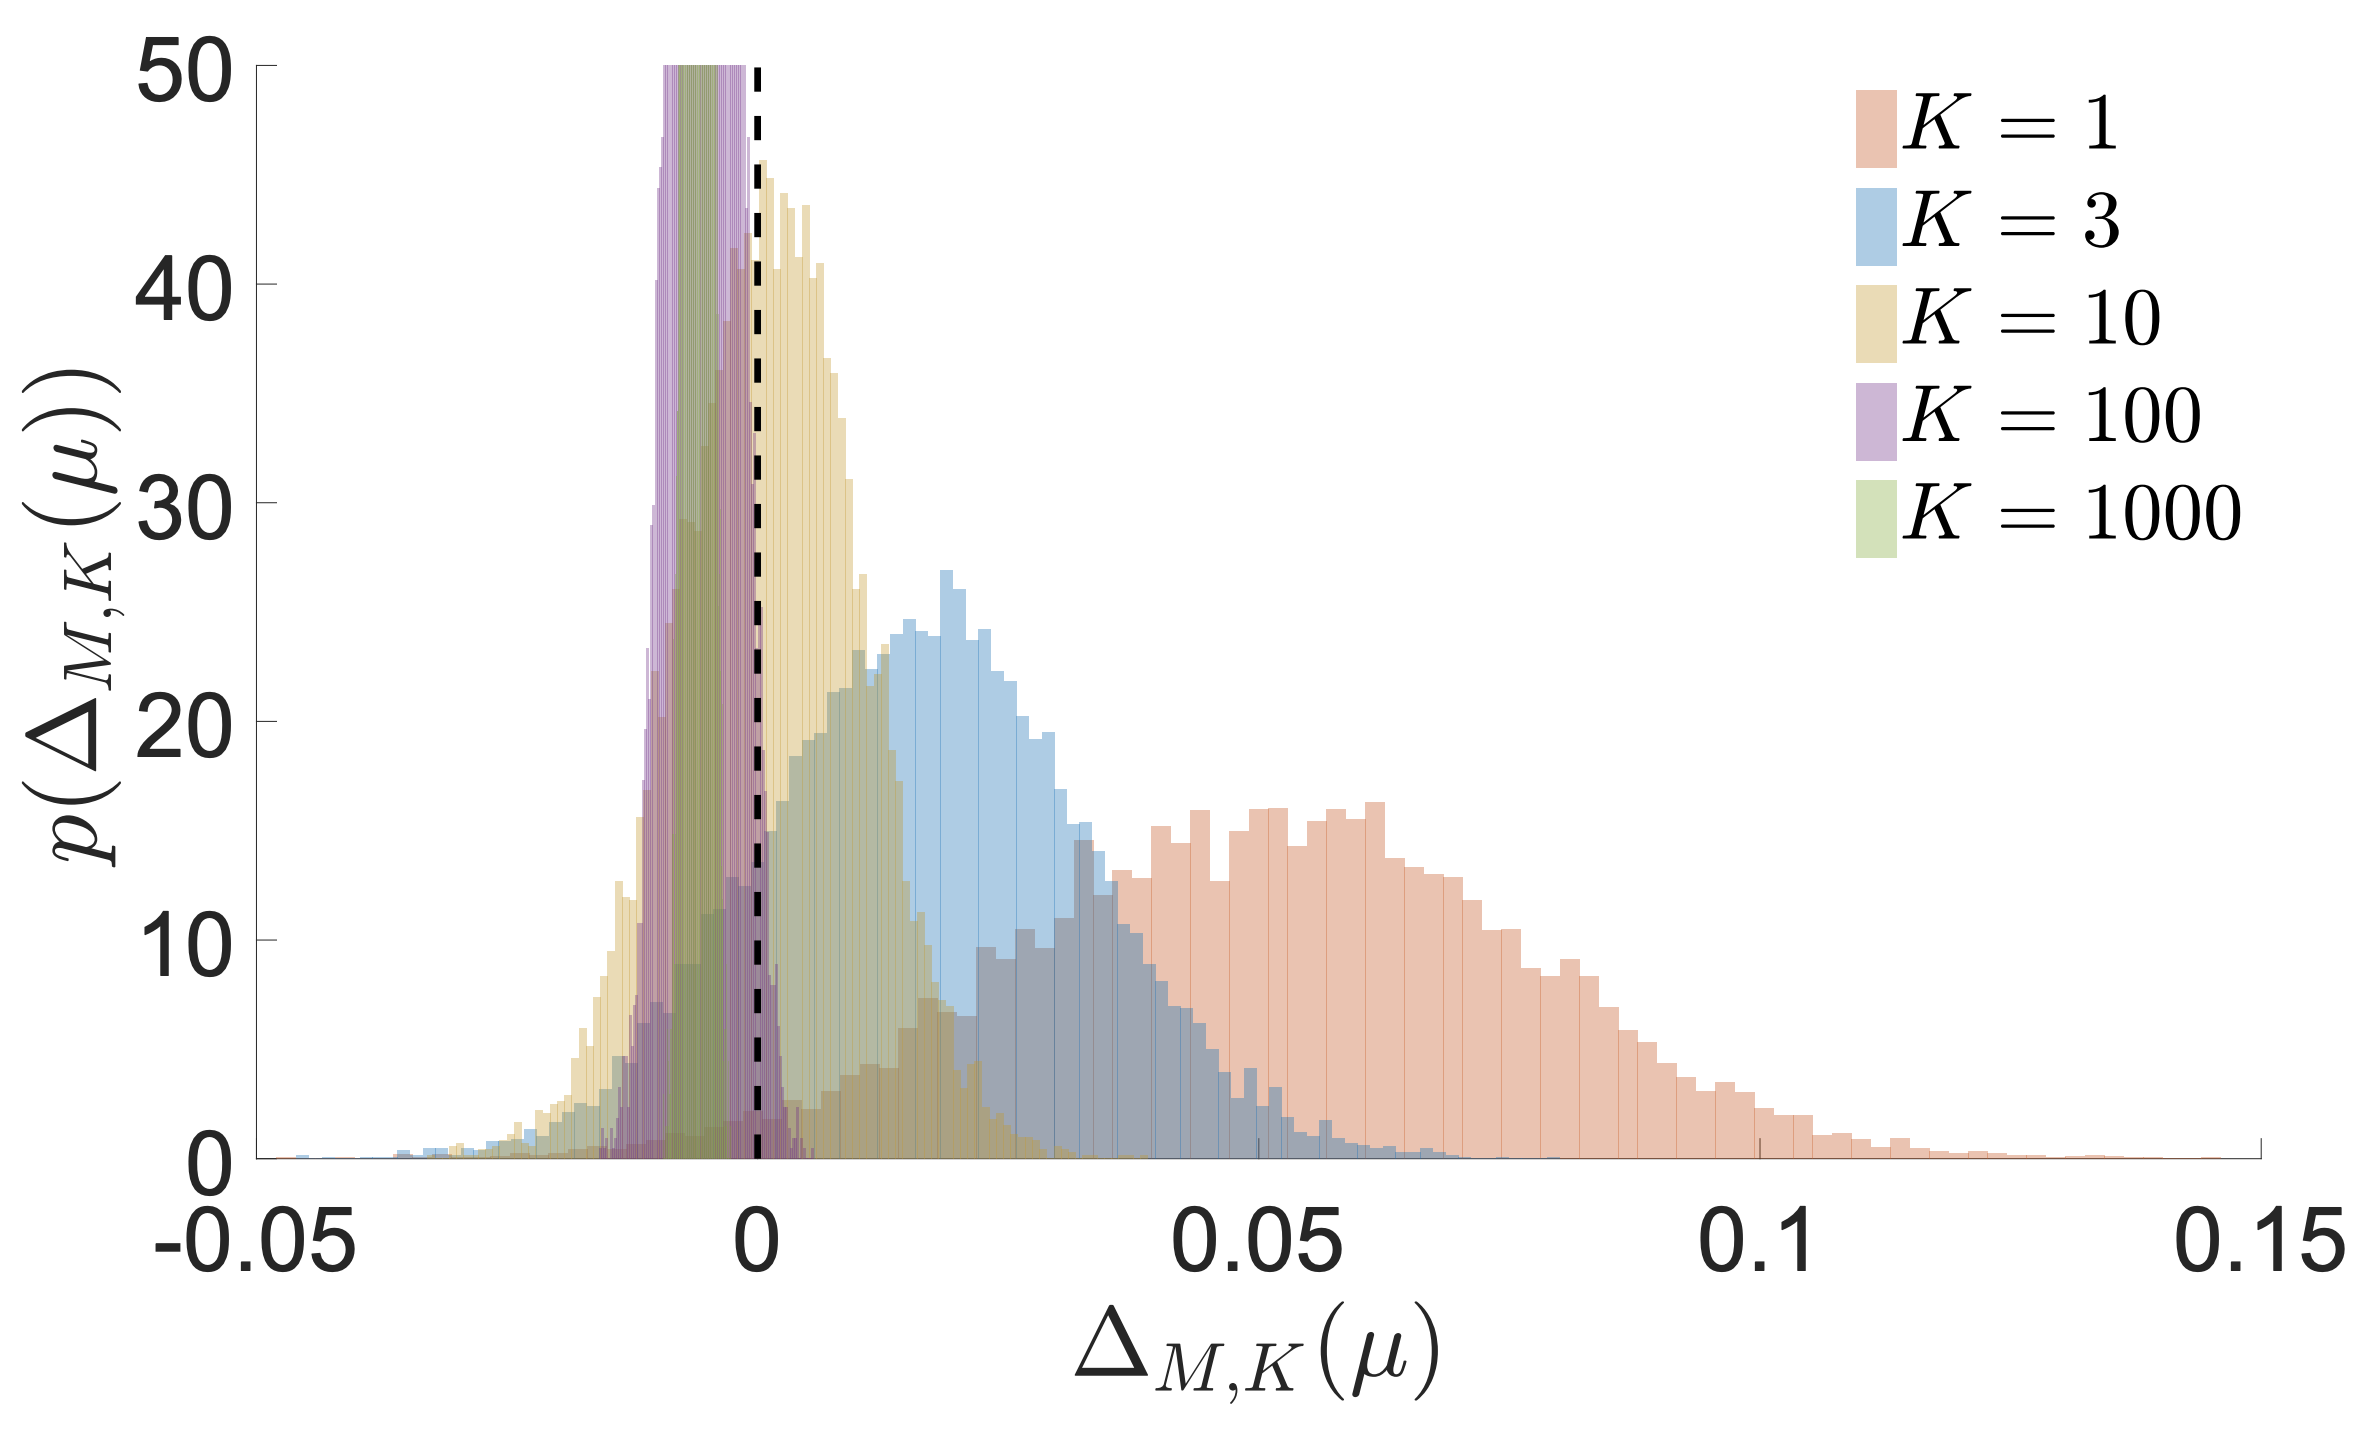
\includegraphics[width=1.\linewidth]{figs/IWAE_SNR_2.png}
			\end{figure}
		\end{minipage}
	\begin{itemize}
		\item IWAE makes the variational bound tighter and extends the class of variational distributions.
		\item Gradient signal becomes really small, training is complicated.
		\item IWAE is a standard quality measure for VAE models.
	\end{itemize}
	\myfootnotewithlink{https://arxiv.org/abs/1802.04537}{Rainforth T. et al. Tighter variational bounds are not necessarily better, 2018}
\end{frame}
%=======
\begin{frame}{Summary}
	\begin{itemize}
		\item The VAE model is an LVM with two neural network: stochastic encoder $q(\bz | \bx, \bphi)$ and stochastic decoder $p(\bx | \bz, \btheta)$.
		\vfill
		\item VAE is not a "true" bayesian model since parameters $\btheta$ do not have a prior distribution.
		\vfill
		\item Standart VAE has several limitations that we will address later in the course.
		\vfill
		\item More powerful decoder in VAE leads to more expressive generative model. However, too expressive decoder could lead to the posterior collapse.
		\vfill
		\item The decoder weakening is a set of techniques to avoid the posterior collapse.
		\vfill
		\item The IWAE could get the tighter lower bound to the likelihood, but the training of such model becomes more difficult.
	\end{itemize}
\end{frame}
\end{document} 